\documentclass{article}
\overfullrule=5pt % mark overfull boxes with black TODO: should remove before handing in

\usepackage{fullpage} % decrease page margins
\usepackage[parfill]{parskip} % change new paragraph indent to new line

\usepackage{tikz} % for drawing
\usetikzlibrary{external} % cache figures to reduce compilation times
\tikzexternalize[prefix=figurecache/] % cache figures into ./figurecache/ (WARNING: directory must exist and pdflatex must be run with --shell-escape)
\usepackage{pgfplotstable}

\usepackage[labelfont=bf]{caption} % for captions
\usepackage{ifthen} % for if/else statements (in plots)

\usepackage{xargs}

\usepackage[block=space,language=australian]{biblatex}
%\DeclareFieldFormat{url}{\url{#1}} % drop URL prefix
\DeclareFieldFormat{urldate}{(visted #1)}
\addbibresource{bib.bib}
%\urlstyle{sf}
\renewcommand{\UrlFont}{\footnotesize\ttfamily}

\usepackage{siunitx}

\usepackage{amsmath}
\usepackage{commath}
\usepackage{todonotes}

\usepackage{amsthm}
\theoremstyle{definition}

\usepackage{hyperref}

\usepackage[sort,noabbrev]{cleveref} % for nicer equation references

\usepackage{xcolor}

\usepackage{pgfplots} % for plotting
\pgfplotsset{compat=1.17}
\usepgfplotslibrary{groupplots}
\usepgfplotslibrary{dateplot}

\newcommand{\Oh}{\mathcal{O}} % Fight me.

\newcommand{\Ltwoerror}[1]{\Vert #1 \Vert_2}

\newcommand\integral[4]{\int_{#3}^{#4} \dif {#2} \, {#1}}
\newcommand\integraltwo[7]{\int_{#4}^{#5} \dif {#2} \int_{#6}^{#7} \dif {#3} \, {#1}}
\usepackage{subcaption}

\usepackage{listings}
\lstset{%
  breaklines=true,
  breakatwhitespace=true,
}

%% \pgfplotsset{compat=newest,
%%     width=6cm,
%%     height=3cm,
%%     scale only axis=true,
%%     max space between ticks=25pt,
%%     try min ticks=5,
%%     every axis/.style={
%%         axis y line=left,
%%         axis x line=bottom,
%%         axis line style={thick,->,>=latex, shorten >=-.4cm}
%%     },
%%     every axis plot/.append style={thick},
%%     tick style={black, thick}
%% }
%% \tikzset{
%%     semithick/.style={line width=0.8pt},
%% }

\title{Semester Project in TMA4212}
\author{
  Thorvald M. Ballestad\\
  Jonas Bueie\\
  Knut Andre Grytting Prestsveen\\
  Herman Sletmoen
}

\begin{document}
\maketitle
\tableofcontents
\newpage

\section{Poisson equation}

In this section, we will solve the one-dimensional Poisson equation
\begin{equation*}
u_{xx} = f(x) \qquad (0 < x < 1)
\end{equation*}
subject to a source term $f(x)$ and different boundary conditions at $x = 0$ and $x = 1$.
First, we will solve it with finite difference methods of first and second order on a uniform grid.
Finally, we solve it on a non-uniform grid and investigate how adaptive mesh refinement (AMR) can be used to obtain accurate solutions by distributing fewer points more cleverly along the grid.
a

First, consider Dirichlet and Neumann boundary conditions at opposite ends and the source given by
\begin{equation*}
u_{xx} = x + \cos(2 \pi x) \qquad (0 < x < 1), \qquad u(0) = a, \qquad u_x(1) = b.
\end{equation*}
The analytical solution is
\begin{equation*}
u(x) = C_1 + C_2 x + \frac{1}{6}x^3 - \frac{1}{4 \pi^2}\cos(2 \pi x)),
\end{equation*}
where the constants $C_1$ and $C_2$ are determined from the boundary conditions.
To solve the equation numerically, we impose a uniform grid of $M+2$ points and step length $h$ defined by
\begin{center}
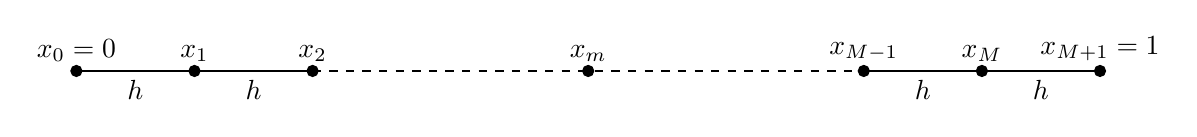
\begin{tikzpicture}
\draw (0,0) -- (3,0);
\draw[dashed] (3,0) -- (10,0);
\draw (10,0) -- (13,0);
\filldraw (0.0,0) circle (2pt) node[anchor=south] {$x_0 = 0$};
\filldraw (1.5,0) circle (2pt) node[anchor=south] {$x_1$};
\filldraw (3.0,0) circle (2pt) node[anchor=south] {$x_2$};
\filldraw (6.5,0) circle (2pt) node[anchor=south] {$x_m$};
\filldraw (10.0,0) circle (2pt) node[anchor=south] {$x_{M-1}$};
\filldraw (11.5,0) circle (2pt) node[anchor=south] {$x_{M}$};
\filldraw (13.0,0) circle (2pt) node[anchor=south] {$x_{M+1} = 1$};
\node[anchor=north] at (0.75, 0) {$h$};
\node[anchor=north] at (2.25, 0) {$h$};
\node[anchor=north] at (10.75, 0) {$h$};
\node[anchor=north] at (12.25, 0) {$h$};
\end{tikzpicture}
.
\end{center}
To generate finite difference methods of both first and second order, we approximate the second derivative at interior points using the forward difference and central difference
\begin{equation*}
\begin{aligned}
u_{xx}(x_m) & = \frac{u_m-2u_{m+1}+u_{m+2}}{h^2} + O(h^1) \qquad && (1 \leq m \leq M) \\
u_{xx}(x_m) & = \frac{u_{m-1}-2u_m+u_{m+1}}{h^2} + O(h^2) \qquad && (1 \leq m \leq M-1).
% TODO: how to use forward difference at point M-1 ???
\end{aligned}
\end{equation*}
To handle the Dirichlet boundary condition $u(0) = a$ at the left edge, we insert the trivial equation
\begin{equation*}
1 \cdot u_0 = a.
\end{equation*}
To handle the Neumann boundary condition $u_x(1) = b$ at the right edge to first or second order, we use
\begin{equation*}
\begin{aligned}
u_x(1) & = \frac{u_{M+1}-u_M}{h} & + & O(h^1) & = b\\
u_x(1) & = \frac{\frac{1}{2}u_{M-1}-2u_M+\frac{3}{2}u_{M+1}}{h} & + & O(h^2) & = b.
\end{aligned}
\end{equation*}
By writing all these equations in $(M+2) \times (M+2)$-matrix form $AU=b$, we obtain for example to second order
\begin{equation*}
\renewcommand{\arraystretch}{1.5} % stretch matrix vertically to make it square
\begin{bmatrix}
1 \\
+1/h^2 & -2/h^2 & +1/h^2 &   \\
  & \ddots & \ddots & \ddots & \\
  &   & +1/h^2 & -2/h^2 & +1/h^2 \\
  &   & +1/2h & -2/h & +3/2h \\
\end{bmatrix}
\begin{bmatrix}
U_0 \\ U_1 \\ \vdots \\ U_M \\ U_{M+1} \\
\end{bmatrix}
=
\begin{bmatrix}
a \\ f(x_1) \\ \vdots \\ f(x_M) \\ b \\
\end{bmatrix}
\end{equation*}

Some remarks:
\begin{itemize}
\item We could handle the Dirichlet boundary condition $u(0) = a$ differently by treating $U_0 = a$ as a known variable.
The system of equations is equivalent if we remove the first row and column of $A$ and the first entries in $U$ and $b$, but simultaneously modify the entry $f(x_1) \rightarrow f(x_1) - a/h^2$.
This approach is more consistent with treating $U_0$ as a known variable, since its precise value is defined by the Dirichlet boundary condition.
However, our approach of inserting a trivial equation $1 \cdot U_0 = a$ keeps the matrix dimensions independent of boundary conditions and makes it easier to reason with how the discretized differential operator represented by $A$ operates on the grid point $U_0$ in the same way it operates on all other grid points.
\item To handle different combinations of Dirichlet and Neumann boundary conditions at the ends, we simply replace the first or last rows of the matrix with the same type of equation.
Note that if the Neumann boundary condition is imposed at the left boundary, the last row of the matrix above would have to be both reversed and negated.
\item When Neumann boundary conditions are imposed at both ends, the solution is determined only up to a constant.
To see this for a general Poisson boundary value problem, note that if $u_{xx} = f(x)$, $u_x(0) = a$ and $u_x(1) = b$, then also $(u+C)_{xx} = f(x)$, $(u+C)_x(0) = a$ and $(u+C)_x(1) = b$ if $C$ is only a constant.
It can also be seen from the general solution for this particular source term that the constant $C_1$ is undetermined when the solution is subject to boundary conditions that involve derivatives only.
In this case, an additional constraint like $u(0) = 0$ must be imposed to define a unique solution.
\end{itemize}
With this in mind, it is now straightforward to solve the Poisson equation subject to any combination of Dirichlet and Neumann boundary conditions at the ends to both first and second order.

\begin{figure}
	\centering
	\begin{tikzpicture}
		\begin{groupplot}[
			group style={group size=2 by 3,horizontal sep=2cm,vertical sep=2cm},
			height=6cm,
			width=0.48\textwidth,
			]
			\nextgroupplot[title={$u(0)=0, \quad u_x(1)=1$},xmode=normal,ymode=normal,xlabel=$x$,ylabel=$u(x)$];
			\addplot [color=red] table [x=x,y=u] {exercise1/dir_neu.dat};
			\addplot [color=black, only marks, mark=x, each nth point=20] table [x=x,y=U] {exercise1/dir_neu.dat};
			\nextgroupplot[xmode=log,ymode=log,xlabel=$h$,ylabel=relative error];
			\addplot [color=red, mark=*] table [x=h,y=disc] {exercise1/dir_neu_err.dat};

			\nextgroupplot[title={$u(0)=1, \quad u(1)=1$},xmode=normal,ymode=normal,xlabel=$x$,ylabel=$u(x)$];
			\addplot [color=red] table [x=x,y=u] {exercise1/dir_dir.dat};
			\addplot [color=black, only marks, mark=x, each nth point=20] table [x=x,y=U] {exercise1/dir_dir.dat};
			\nextgroupplot[xmode=log,ymode=log,xlabel=$h$,ylabel=relative error];
			\addplot [color=red, mark=*] table [x=h,y=disc] {exercise1/dir_dir_err.dat};

			\nextgroupplot[title={$u_x(0)=0, \quad u_x(1)=1/2$},xmode=normal,ymode=normal,xlabel=$x$,ylabel=$u(x)$,scaled ticks=false, tick label style={/pgf/number format/fixed}];
			\addplot [color=red] table [x=x,y=u] {exercise1/neu_neu.dat};
			\addplot [color=black, only marks, mark=x, each nth point=20] table [x=x,y=U] {exercise1/neu_neu.dat};
			\nextgroupplot[xmode=log,ymode=log,xlabel=$h$,ylabel=relative error];
			\addplot [color=red, mark=*] table [x=h,y=disc] {exercise1/neu_neu_err.dat};
		\end{groupplot}
	\end{tikzpicture}
	\caption{\label{fig3}
		Analytical and numerical solutions (left) and convergence plots (right) for solutions to the Poisson equation subject to three different boundary conditions.
	}
\end{figure}

\iffalse
\begin{equation*}
\renewcommand{\arraystretch}{2.8} % stretch matrix vertically to make it square
\begin{bmatrix}
-2/h^2 & +1/h^2  & 0 & \cdots & 0 \\
+1/h^2  & -2/h^2 & +1/h^2  & \ddots & \vdots \\
0 & \ddots & \ddots & \ddots & 0 \\
\vdots & \ddots & +1/h^2 & -2/h^2 & +1/h^2\\
0 & \cdots & +1/2h & -2/h & +3/2h  \\
\end{bmatrix}
\begin{bmatrix}
U_1 \\ U_2 \\ \vdots \\ U_M \\ U_{M+1} \\
\end{bmatrix}
=
\begin{bmatrix}
f(x_1) - \alpha/h^2 \\ f(x_2) \\ \vdots \\ f(x_M) \\ \sigma \\
\end{bmatrix}
\end{equation*}






Note that when Neumann-Neumann boundary conditions are imposed, $C_1$ is undetermined and so the solution is determined only up to a constant.
To obtain a first order approximation of the second derivative at 





with the source term $f(x) = x + \cos(2 \pi x)$, subject to different kinds of boundary conditions
\begin{equation*}
\begin{aligned}
u(0) &= a, &\quad u(1) &= b &\qquad& \text{(Dirichlet-Dirichlet)} \\
u_x(0) &= a, &\quad u_x(1) &= b &\qquad& \text{(Neumann-Neumann)} \\
u(0) &= a, &\quad u_x(1) &= b &\qquad& \text{(Dirichlet-Neumann)}. \\
\end{aligned}
\end{equation*}


Inner points:
\begin{equation*}
\frac{U_{m+1} - 2 U_m + U_{m-1}}{h^2} = f(x_m)
\end{equation*}
Dirichlet, left:
\begin{equation*}
u(0) = U_0
\end{equation*}
Von-Neumann, left, 2nd order:
\begin{equation*}
u_x(0) \approx -\frac{(3/2)U_0 -2U_1 + (1/2)U_2}{h}
\end{equation*}
\fi


\begin{figure}
  \centering
  \begin{tikzpicture}
\begin{loglogaxis}[
  title=Error functions,
  xlabel={$M$},
  ylabel={$e_l$},
  legend pos=south west,
  ]

  \addplot table[y index=1] {exercise1/a_error.dat}
  coordinate [pos=0.24] (A)
  coordinate [pos=0.8] (B);
  \addplot table[y index=2] {exercise1/a_error.dat};
  \addplot table[y index=3] {exercise1/a_error.dat};

  \draw (A) -| (B)
  node [pos=0.25, anchor=south] {1}  %% Random value
  node [pos=0.75, anchor=west] {-1};

  \legend{$L_2$ discrete, $L_2$ continous step, $L_2$ continous interpolatino};
\end{loglogaxis}
\end{tikzpicture}

  \caption{Nice fig}
\end{figure}


\clearpage
\section{Heat equation in one dimension}


\clearpage
\section{Laplace equation in two dimensions}
In this section, we will solve the two-dimensional Laplace equation on a quadratic domain
\begin{equation}
    u_{xx} + u_{yy} = 0, \, (x,y) \in \Omega := [0,1]^2,
    \label{ex3:eq:laplace}
\end{equation} with boundary conditions on the edges of $\Omega$
\begin{equation*}
    \begin{split}
        u(0,y) &= 0,\\
        u(1,y) &= 0,\\
        u(x,0) &= 0,\\
        u(x,1) &= \sin(2\pi x).\\
    \end{split}
\end{equation*}
We will solve this equation numerically using a five point stencil, but first, we solve it analytically to provide a reference solution which can be compared with the numerical one.

The solution of equation \ref{ex3:eq:laplace} can be found by separation of variables.
First, asssume that we can write
\begin{equation*}
    % I used these names, but I think it's more common with capital X and Y or something.
    % I'm open for discussions of this.
    u(x,y) = \alpha(x) \beta(y),
\end{equation*}
which implies that
\begin{equation*}
    u_{xx} + u_{yy} =  \alpha''(x) \beta(y) + \alpha(x) \beta''(y) = 0,
\end{equation*}
where the prime markers $'$ denote differentiation of the single variable functions $\alpha(x)$ and $\beta(y)$.
Rearranging, we get that
\begin{equation*}
    \frac{\alpha''(x)}{\alpha(x)} = \frac{\beta''(y)}{\beta(y)} = c
\end{equation*}
must be constant, since $\alpha$ and $\beta$ are functions of indepentent variables.
Thus, we have two second order differential equations
\begin{equation*}
    \begin{split}
        \alpha''(x) - c\alpha(x) &= 0, \\
        \beta''(x) - c\beta(x) &= 0,
    \end{split}
\end{equation*}
with boundary conditions
\begin{equation*}
    \begin{split}
    \alpha(0) = \alpha(1) = \beta(0) = 0,\\
    \alpha(x)\beta(1) = \sin(2\pi x).
    \end{split}
\end{equation*}

Setting $\beta(1)$ to $1$ yields $\alpha(x) = \sin(2\pi x)$, so that $\alpha''(x) = -4\pi^2\alpha(x)$ where $y = 1$, we find that $c = -4\pi^2$.
Solving the equation for $\beta(y)$, we find that
\begin{equation*}
    \beta(y) = b_1 e^{\sqrt{c} y} + b_2 e^{-\sqrt{c} y}.
\end{equation*}
Inserting $c = 4\pi$ and the boundary condtitions $\beta(0) = 0$ and $\beta(1) = 1$, we get
\begin{equation*}
    \beta(y) = \frac{\sinh(2\pi y)}{\sinh(2\pi)},
\end{equation*}
and finally
\begin{equation*}
    u(x,y) = \frac{\sin(2\pi x) \cdot \sinh(2\pi y)}{\sinh(2\pi)}.
\end{equation*}

Numerically, we can solve this equation by dividing the domain $\Omega$ into a grid.
That is, we divide the interval $x \in [0,1]$ and $y \in [0,1]$ into $M$ and $N$ parts, respectively, so that the domain contains $M * N$ points, in which we will approximate the solution to equation \ref{ex3:eq:laplace}.

Rewriting Laplace's equation using central differences, we get
\begin{equation*}
    \begin{split}
    % This notation is indonsistent with task 1, but it is explicit 
    % regarding in which points we evaluate the function.
    % TODO: What do you people think?
    \partial^2_x u(x_m, y_n) 
        &= \frac{1}{h^2}[u(x_{m-1},y_n) + 2u(x_m,y_n) + u(x_{m+1},y_n)] + O(h^2)\\
        &= \frac{1}{h^2}\delta^2_x u(x_m,y_n),\\
    \end{split}
\end{equation*}
\begin{equation*}
    \begin{split}
    \partial^2_y u(x_m, y_n) 
        &= \frac{1}{k^2}[u(x_{m},y_{n-1}) + 2u(x_m,y_n) + u(x_{m},y_{n+1})] + O(k^2)\\
        &= \frac{1}{h^2}\delta^2_y u(x_m,y_n),\\
    \end{split}
\end{equation*}
where $(x_m, y_n)$ denote the point $(m,n)$ in the grid. 
%$i = 0,\ldots M_x$, and $j = 0,\ldots, M_y$.
Adding these expressions, and naming our approximated solution $U(m,n) := u(x_m,y_n)$, we find that the function $u_{xx} + u_{yy}$ can be approximated 
\begin{equation*}
    0 = u_{xx}(x_m,y_n) + u_{yy}(x_m,y_n)
    \approx \frac{1}{h^2}\delta^2_x U(m,n) + \frac{1}{k^2}\delta^2_y U(m,n),
\end{equation*}
or, simplifying the notation as shown in figure % TODO: \ref{ex3:fig:stencil}
,
\begin{equation*}
    U_{above} + U_{below} + U_{left} + U_{right} - 4_{center} = 0.
\end{equation*}
This stencil can be used to approximate the value of $U(x_m, y_n) = U_{center}$ for all points $(x_m, y_n)$ in the grid.


\clearpage
\section{Linearized Korteweg-De Vries equation in one dimension}

KdV equation:
\begin{equation}
u_t + (1+\pi^2)u_x + u_{xxx} = 0
\end{equation}

\begin{figure}
\begin{tikzpicture}
\begin{axis}[
areaplot1/.style={fill opacity=0.50, fill=green, mark=none},
areaplot2/.style={fill opacity=0.50, fill=red, mark=none},
width=17cm,
height=12cm,
view={-28}{+30},
xlabel={$x$},
ylabel={$t$},
zmin=0,
ymajorgrids,
xmajorgrids,
xtick distance=0.50,
ytick distance=0.25,
legend cell align={left},
]
\pgfplotsinvokeforeach{5,4,...,1}{
	% Filled version
	% \addplot3 [areaplot1] table [x index=0,y expr={#1/5},z expr=\thisrowno{#1}+1] {exercise4/timeevol.dat} \closedcycle;
	% \pgfmathparse{int(round(5+#1))};
	% \pgfmathtruncatemacro\mymacro{round(5+#1)};
	% \addplot3 [areaplot2] table [x index=0,y expr={#1/5},z expr=\thisrowno{\mymacro}+1] {exercise4/timeevol.dat} \closedcycle;
	% \node[draw] at (0, 2) {\mymacro}; % for debug

	% Non-filled version
	\addplot3 [fill=gray, opacity=0.75, mark=none, draw=gray!80!black, thick] table [x index=0,y expr={(#1-1)/(5-1)},z expr=\thisrowno{#1}+1] {exercise4/timeevol.dat} \closedcycle;
	\ifthenelse{\equal{#1}{5}}{\addlegendentry{$u(x,t) = \sin(\pi(x-t))$}}{}
	\pgfmathparse{int(round(5+#1))};
	\pgfmathtruncatemacro\mymacro{round(5+#1)};
	\addplot3 [mark=none, color=red, thick] table [x index=0,y expr={(#1-1)/(5-1)},z expr=\thisrowno{\mymacro}+1] {exercise4/timeevol.dat};
	\ifthenelse{\equal{#1}{5}}{\addlegendentry{$U(x_m,t_n)$}}{}
	\node[draw] at (0, 2) {\mymacro}; % for debug
}
\end{axis}
\end{tikzpicture}
\end{figure}

Theta method:
\begin{equation}
\frac{u_m^{n+1} - u_m^n}{k} = (1-\theta) F(u^n) + \theta F(u^{n+1})
\end{equation}
where
\begin{equation}
F(u^n) = -(1+\pi^2) \frac{u_{m+1}^n-u_{m-1}^n}{2h} - \frac{u_{m+3}^n-3u_{m+1}^n+3u_{m-1}^n-u_{m-3}^n}{8h^3}
\end{equation}
$\theta = 0$ is forward Euler, $\theta = 1/2$ is Crank-Nicholson, $\theta = 1$ is backward Euler.

Separation of variables:
\begin{equation}
u(x, t) = X(x) T(t)
\end{equation}
Insert into KdV equation to get $T = A e^{zt}$.
$X(x)$ is periodic, so expand it in a Fourier series:
\begin{equation}
X(x) = \sum_k C_k e^{ikx}
\end{equation}
The general solution is then
\begin{equation}
u(x, t) = \sum_k C_k e^{kt} e^{ikx}
\end{equation}
so
\begin{equation}
u_m^n = \sum_k C_k e^{kt_n} e^{ikx_m}
\end{equation}
With constant time steps, $t_n = nk$, we can write
\begin{equation}
u_m^n = \sum_k C_k G^n e^{ikx_m}
\end{equation}
Consider a general term in the series $u_m^n = G^n e^{ikx_m}$. Insert into discretized KdV equation to get
\begin{equation}
\frac{G-1}{k} = [(1-\theta)+\theta G] [-(1+\pi^2) \frac{e^{iqh}-e^{-iqh}}{2h} - \frac{e^{3iqh}-e^{-3iqh}-3(e^{iqh}-e^{-iqh})}{8h^3}]
\end{equation}
Expand using Euler's identity to get
\begin{equation}
\frac{G-1}{k} = i [(1-\theta)+\theta G] [-(1+\pi^2) \frac{\sin(qh)}{h} - \frac{\sin^3(qh)}{h^3}]
\end{equation}
$\theta = 0$ gives $|G| > 1$ (unstable), but $\theta = 1/2$ gives $|G| = 1$ (stable)! (unconditionally)

Proof of conserved norm:
Due to periodicity (if one is very pedantic, one can obtain this by separation of variables)
\begin{equation}
	u(x, t) = \sum_n c_n(t) e^{i k_n x}
\end{equation}
Insert into the KdV equation to get
\begin{equation}
	\sum_n \left\{ \dot{c}_n(t) + i [(1+\pi^2)k_n - k_n^3] c_n(t) \right\} e^{i k_n x}= 0
\end{equation}
For the sum to be $0$, each term inside the curly brackets must vanish, so
\begin{equation}
	c_n(t) = c_n(0) \exp{\left\{ i [(1+\pi^2)k_n - k_n^3] t \right\} }
\end{equation}
Thus,
\begin{equation}
\begin{split}
\int_{-1}^{+1} \dif x \left| u(x,t) \right|^2 &= \int_{-L/2}^{+L/2} \sum_{m,n} c_m(t) c_n^*(t) \exp{(i k_m x)} \exp{(-i k_n x)} \\
                                              &= \sum_{m,n} c_m(t) c_n^*(t) \underbrace{\int_{-L/2}^{+L/2} \exp{(i(k_m-k_n)x)}}_{L \delta_{m n}} \\
											  &= L \sum_n \left| c_m(t) \right|^2 \\
											  &= L \sum_n \left| c_m(0) \right|^2 \\
											  &= \int_{-L/2}^{+L/2} \dif x \left| u(x,0) \right|^2,
\end{split}
\end{equation}
so the spatial $L_2$-norm is preserved over time.


\clearpage
\section{Poisson equation in one dimension finite element method}

\newcommand\basisexpand[2]{\sum_{i=0}^{M+1} #1_i \varphi_i(#2)}

In this section, we will again solve the Poisson equation
\begin{equation}
	-\pd[2]{u}{x} = f(x), \quad u(a) = \alpha, \quad u(b) = \beta, \quad (a \leq x \leq b)
	\label{poisson_equation2}
\end{equation}
subject to Dirichlet conditions, but this time using finite elements instead of finite differences.

\subsection{Analytical solution}

The solution to the Poisson equation is the same as in \ref{poisson_analytical_solution}, but with $f(x) \rightarrow -f(x)$, so that
\begin{equation}
u(x) = C_1 + C_2 x - \int^x \dif x' \int^{x'} \dif x'' f(x'').
\label{poisson_analytical_solution2}
\end{equation}

\subsection{Weak formulation for the exact solution}

To derive a finite element method, we first split the solution into two terms
\begin{equation}
	u(x) = \hat{u}(x) + r(x), \quad \text{with} \quad \hat{u}(a) = \hat{u}(b) = 0 \quad \text{and} \quad r(x) = \alpha \frac{x-b}{a-b} + \beta \frac{x-a}{b-a}.
	\label{splitting_exact}
\end{equation}
Note that $u''(x) = \hat{u}''(x)$ and $r(a) = \alpha$ and $r(b) = \beta$.
The purpose of this splitting is that $\hat{u}$ solves \ref{poisson_equation2} with homogenuous Dirichlet boundary conditions, while $r(x)$ \textbf{lifts} the values at the boundaries to satisfy the inhomogenuous boundary conditions.

Now insert \ref{splitting_exact} into \cref{poisson_equation2}, multiply it by a \textbf{trial function} $v(x)$ and integrate both sides from $a$ to $b$.
We let $v(a) = v(b) = 0$ and use integration by parts on the left, dropping the boundary term term $-[u'(x) v(x)]_a^b$.
This gives the \textbf{weak formulation} of the problem:
\newcommand{\weakform}[3]{
\text{Find} \,\, \hat{#1}(x) \,\, \text{such that}
\quad
\integral{\hat{#1}'(x) #2'(x)}{x}{a}{b} = \integral{f(x) #2(x)}{x}{a}{b} - \integral{#3'(x) #2'(x)}{x}{a}{b}
\quad
\text{for all} \,\, #2(x)
}
\begin{equation}
	\weakform{u}{v}{r}.
	\label{weak_form_exact}
\end{equation}
The weak formulation \ref{weak_form_exact} is equivalent to the original boundary value problem \ref{poisson_equation2}.
Any $u(x)$ that solves \ref{poisson_equation2} also solves \ref{weak_form_exact}, and it is possible to show that the converse is also true.

\subsection{Weak formulation for the approximate solution}

We have not made any approximations yet.
The approximation lies in seeking a solution $U(x) \approx u(x)$ that belongs to a function space different from the one in which the exact solution $u(x)$ belongs.
Here, we suppose $U(x)$ lies in the space of piecewise linear functions.
We will then repeat the process above to derive a weak formulation for $U(x)$, similarly as for the exact solution.

To see how this works, we first divide the interval $[a, b]$ into the grid
\begin{equation}
	a = x_0 < x_1 < \dots < x_M < x_{M+1} = b
	\label{fem_grid}
\end{equation}
and let $U(x)$ be piecewise linear in each \textbf{finite element} $[x_i, x_{i+1}]$.
Similarly to $u(x)$, we split the approximate solution into
\begin{equation}
	U(x) = \hat{U}(x) + R(x), \quad \text{with} \quad \hat{U}(a) = \hat{U}(b) = 0 \quad \text{and} \quad R(x) = 
	\begin{cases}
		\alpha \dfrac{x_1-x}{x_1-a} & (a \leq x \leq x_1)   \\
		0                           & (x_1 \leq x \leq x_M) \\
		\beta  \dfrac{x-x_M}{b-x_M} & (x_M \leq x \leq b)   \\
	\end{cases}
	.
	\label{weak_form_approximate}
\end{equation}
Now again insert \ref{weak_form_approximate} into \ref{poisson_equation2}, multiply by a trial function $V(x)$ that vanishes at $a$ and $b$, integrate from $a$ to $b$ and drop a boundary term.
This leads to the weak formulation for the approximate solution:
\begin{equation}
	\weakform{U}{V}{R}.
	\label{weak_form_approximate}
\end{equation}

\subsection{Numerical solution}

To obtain a matrix equation for approximate solution $U(x)$, the next step is to expand
\begin{equation}
	\hat{U}(x) = \basisexpand{\hat{U}}{x} \quad \text{and} \quad V(x) = \basisexpand{V}{x}
	\label{expansion}
\end{equation}
in a basis for the approximate solution function space, namely the piecewise linear functions on the grid \ref{fem_grid}.
The most natural basis for this space are the functions
\begin{equation}
	\varphi_i(x) = 
	\begin{cases}
		(x - x_{i-1})/(x_i - x_{i-1}) & \text{if}        \,\, x_{i-1} \leq x \leq x_i     \\
		(x_{i+1} - x)/(x_{i+1} - x_i) & \text{if}        \,\, x_i     \leq x \leq x_{i+1} \\
		0                             & \text{otherwise} \\
	\end{cases}
	=
	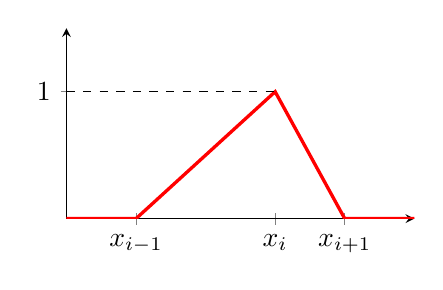
\begin{tikzpicture}[baseline={([yshift=-.5ex]current bounding box.center)}]
	\begin{axis}[width=6cm,height=4cm,xmin=0, xmax=5, ymax=1.5,
	xtick={1,3,4}, xticklabels={$x_{i-1}$,$x_i$,$x_{i+1}$},
	ytick={0,1},
	axis lines=middle
	]
	\addplot [red, very thick] coordinates {
		(-2,0)
		(1,0)
		(3,1)
		(4,0)
		(6,0)
	};
	\addplot [dashed] coordinates {(0,1) (3,1)};
	\end{axis}
	\end{tikzpicture}
	\label{basisfunction}
	.
\end{equation}
With this basis, the coefficients $\hat{U}_i = \hat{U}(x_i)$ are simply the values at the grid points, making it straightforward to plot the solution.
Inserting this expansion into \ref{weak_form_approximate} gives
\begin{equation*}
\begin{split}
	\sum_{i, j} \hat{U}_i V_j \integral{\varphi'_i(x) \varphi'_j(x)}{x}{a}{b}
	&= \sum_j V_j \integral{\varphi_j(x) f(x)}{x}{a}{b} \\
	&- a \sum_j V_j \integral{\varphi'_0(x) \varphi'_j(x)}{x}{a}{b}
	- b \sum_j V_j \integral{\varphi'_{M+1}(x) \varphi'_j(x)}{x}{a}{b}.
\end{split}
\end{equation*}
We can write this as the neat matrix equation $V^T A \hat{U} = V^T F$ by introducing
\begin{equation*}
	\hat{U} = [\hat{U}_1, \dots, \hat{U}_M]^T,
	\quad
	V = [V_1, \dots, V_M]^T,
	\quad
	A_{ij} = \integral{\varphi'_i(x) \varphi'_j(x)}{x}{a}{b}
	\quad \text{and} \quad
	F_j = \integral{\varphi_j(x) f(x)}{x}{a}{b}.
\end{equation*}
for $0 \leq i, j \leq M+1$.
Since this must hold for \emph{any} $V(x)$ and thus $V$, we must have
\begin{equation}
	A \hat{U} = F.
	\label{fem_matrixeq}
\end{equation}
This is the matrix equation we will solve to find $U(x)$.
After finding $\hat{U}$, we simply sum \ref{expansion} and add $R(x)$ to find $U(x)$.
Note that our particular choice of basis \ref{basisfunction} gives the convenient property $U(x_i) = U_i$, so summing is not necessary in practice.

To solve \ref{fem_matrixeq}, we must first calculate the so-called \textbf{stiffness matrix} $A$ and the \textbf{load vector} F.
The former involves only the known basis functions and gives nonzero entries
\begin{align*}
	A_{00} = \frac{1}{x_1 - x_0}                           \qquad & \qquad A_{M+1 M+1} = \frac{1}{x_{M+1}-x_M} \\
	A_{ii} = \frac{1}{x_i-x_{i-1}} + \frac{1}{x_{i+1}-x_i} \qquad & \qquad A_{i i+1} = A_{i+1 i} = \frac{1}{x_{i+1}-x_i}.
\end{align*}
The latter involves integrals over an arbitrary source function $f(x)$ times the basis functions $\varphi_j(x)$.
This integral must be approximated numerically and should be split from $x_{i-1}$ to $x_i$ and $x_i$ to $x_{i+1}$ to properly handle the spike in $\varphi_j(x)$ at $x_j$.
(TODO: comment on numerical integration procedure, Gaussian integration)

We now impose $\hat{U}(a) = \hat{U}(b) = 0$ by removing the first and last entries in the matrix equation \emph{after} calculating the entire $(M+2) \times (M+2)$ system described above.
This gives an $M \times M$ equation.
Then we construct $U$ by appending $\alpha$ and $\beta$ at the beginning and end of the $M$-vector $\hat{U}$.

\newcommand\plotseries[5]{
\pgfplotstablegetrowsof{#1-step0.dat}
\pgfmathsetmacro{\MA}{\pgfplotsretval}
\pgfplotstablegetrowsof{#1-step1.dat}
\pgfmathsetmacro{\MB}{\pgfplotsretval}
\pgfplotstablegetrowsof{#1-step2.dat}
\pgfmathsetmacro{\MC}{\pgfplotsretval}

\begin{tikzpicture}
\begin{groupplot}[
	group style={group size=3 by 2, horizontal sep=0.1cm, vertical sep=0.1cm},
	width=6.4cm,
	xtick={#4, #5}, minor xtick=data,
]

\nextgroupplot[height=3cm, xticklabels={,,}, xtick={#4, #5}, minor xtick=data, ymin=0, ymax=1.2, ytick={0, 1}, minor ytick={0.5}, title={$M=\MA$}, ylabel={$E/E_{\text{max}}$}];
\addplot [ybar interval, fill=red] table [x=x, y=E] {#1-step0.dat}; % errors
\addplot [black, dashed] table [y=refE] {#1-step0.dat}; % reference error line
\nextgroupplot[height=3cm, xticklabels={,,}, xtick={#4, #5}, minor xtick=data, ymin=0, ymax=1.2, ytick={0, 1}, minor ytick={0.5}, title={$M=\MB$}, yticklabels={,,}];
\addplot [ybar interval, fill=red] table [x=x, y=E] {#1-step1.dat}; % errors
\addplot [black, dashed] table [y=refE] {#1-step1.dat}; % reference error line
\nextgroupplot[height=3cm, xticklabels={,,}, xtick={#4, #5}, minor xtick=data, ymin=0, ymax=1.2, ytick={0, 1}, minor ytick={0.5}, title={$M=\MC$}, yticklabels={,,}];
\addplot [ybar interval, fill=red] table [x=x, y=E] {#1-step2.dat}; % errors
\addplot [black, dashed] table [y=refE] {#1-step2.dat}; % reference error line

\nextgroupplot[xlabel=$x$];
\addplot [draw=none] table [x=x, y=U] {#1-step0.dat}; % hidden dummy plot (just for ticks)
\addplot [blue, domain=#4:#5, samples=300, line width=1pt, black] {#2}; % analytical
\addplot [black, mark=*, mark size=1.0, red, line width=0.5pt] table [x=x, y=U] {#1-step0.dat}; % numerical

\nextgroupplot[xlabel=$x$, yticklabels={,,}];
\addplot [draw=none] table [x=x, y=U] {#1-step1.dat}; % hidden dummy plot (just for ticks)
\addplot [blue, domain=#4:#5, samples=300, line width=1pt, black] {#2}; % analytical
\addplot [black, mark=*, mark size=1.0, red, line width=0.5pt] table [x=x, y=U] {#1-step1.dat}; % numerical

\nextgroupplot[xlabel=$x$, yticklabels={,,}];
\addplot [draw=none] table [x=x, y=U] {#1-step2.dat}; % hidden dummy plot (just for ticks)
\addplot [blue, domain=#4:#5, samples=300, line width=1pt, black] {#2}; % analytical
\addplot [black, mark=*, mark size=1.0, red, line width=0.5pt] table [x=x, y=U] {#1-step2.dat}; % numerical
\end{groupplot}
\end{tikzpicture}
}

\newcommand\figureseries[3]{
\begin{figure}
\centering
$f(x) = -2$
\medskip \medskip
\plotseries{#1/f1}{x^2}{}{0}{1} \\
\medskip \medskip \medskip \medskip
$f(x) = (40000x^2 - 200) \exp(-100x^2)$
\medskip \medskip 
\plotseries{#1/f2}{exp(-100) - exp(-100*x^2)}{}{-1}{1} \\
\end{figure}
\begin{figure}
\ContinuedFloat % split over two pages
\centering
$f(x) = (4000000x^2 - 2000) \exp(-1000x^2)$
\medskip \medskip
\plotseries{#1/f3}{exp(-1000) - exp(-1000*x^2)}{}{-1}{1} \\
\medskip \medskip \medskip \medskip
$f(x) = 2x^{-4/3}/9$
\medskip \medskip
\plotseries{#1/f4}{x^(2/3)}{}{0}{1}
\caption{\label{#2}#3}
\end{figure}
}

\subsubsection{Uniform refinement}

We test our method on four problems, shown in \cref{femumr}, with uniform elements $x_i - x_{i-1} = (b-a)/(M+1)$.

The approximate solutions resembles the exact solution with few points.
For the symmetric Gaussian problems, it is vital to choose an odd number of grid points to capture the spike in the center.
In the final problem, the source function diverges at the left boundary, but the numerical integration is still able to find a good numerical solution.

In all but the first problem, errors distribute non-evenly across the elements.
Computational resources are wasted by using many points in areas where the solution varies slowly.
These resources would be better spent by increasing the grid resolution in the areas where the error is large.
This is the motivation for turning to adaptive refinement and non-uniform grids.

\figureseries{exercise5/data/UMR}{femumr}{Uniform refinement}

\subsubsection{Adaptive refinement}
\label{fem_amr_section}

Motivated by the uneven error distribution from using uniform elements, we will now do adaptive refinement, similarly to what we did in \cref{ex1_amr_section}.
We start with a uniform grid and successively split those elements on which the error is largest.
Contrary to what we did in \cref{ex1_amr_section}, we will not split only \emph{one} element between each iteration of the numerical solution, but split \emph{all} elements on which the error is greater than some reference error.
This leaves us with less control over the number of elements, but in return we will see that the error strictly decreases in each iteration, eliminating the oscillating error in \cref{amr_convergence_plot}.

This time, we use two strategies that both involve the exact error:
\begin{enumerate}
\item \textbf{Average error strategy:} Split the interval $[x_m, x_{m+1}]$ with error 
\begin{equation*}
\Ltwoerror{u(x)-U(x)} > 0.99 \, \dfrac{\Ltwoerror{u(x)-U(x)}}{N},
\end{equation*}
where $N$ is the number of intervals.
The safety factor $0.99 \approx 1$ ensures that intervals are split also when all errors are equal (up to machine precision), so the procedure does not halt unexpectedly.
\item \textbf{Maximum error strategy:} Split the interval $[x_m, x_{m+1}]$ with error
\begin{equation*}
\Ltwoerror{u(x)-U(x)} > 0.70 \, \max{\Ltwoerror{u(x)-U(x)}},
\end{equation*}
where $N$ is the number of intervals.
\end{enumerate}

In \cref{femamr}, we show how the errors distribute on the same four problems as in \cref{femumr} using the average error strategy.

Observe how only elements with large error are refined, while others are left untouched.
In the symmetric Gaussian problems, the refinement ensure that the middle element is split immediately if we do not start with a grid point at the peak.
In the final problem, we see that it is almost only elements close to the left boundary where the source diverges that needs to be refined.

As discussed above, we see that the errors in the first problem distribute evenly on the initial uniform grid.
This shows the importance of the safety factor $0.99$ in the average error strategy.
Without it, precision issues would make some elements skip the refinement criterion.

\subsubsection{Comparison of convergence}

Finally, in \cref{femconvergence}, we compare the convergence of uniform and adaptive refinement strategies.

In all problems, adaptive refinement yields greater or equal accuracy for a given number of elements compared to uniform refinement.
This is in contrast to what was the case for the finite difference method in \cref{amr_convergence_plot}, where adaptive refinement gave errors only comparable and usually larger than those from uniform refinement.
It is only in the first problem that all strategies behave identically, as the errors here distribute evenly across the elements.

By splitting multiple intervals between each iteration of the numerical solution, we have eliminated the oscillating error pattern in \cref{amr_convergence_plot}.
Now the error strictly decreases between each refinement of the grid.
This suggests that the oscillating pattern is due to refinements where intervals with large error are present even after refining the element with greatest error.
For example, it would be a bad idea to refine only \emph{one} element in the first problem in \cref{femamr}, where errors are even across the elements.

\figureseries{exercise5/data/AMR}{femamr}{Adaptive refinement, average strategy}

\begin{figure}[h!]
\centering
\begin{tikzpicture}
\begin{groupplot}[
	group style={group size=2 by 2, horizontal sep=1.5cm, vertical sep=2.5cm},
	xmode=log, ymode=log,
	width=8cm, height=7cm, 
	legend entries={uniform, adaptive (avg.), adaptive (max)},
	log basis x=2, xticklabel=\pgfmathparse{2^\tick}\pgfmathprintnumber\pgfmathresult,
]
\pgfplotsinvokeforeach {1,2,3,4} {
	\ifthenelse{\equal{#1}{1}}{
		\nextgroupplot[ylabel=error,title={$f(x) = -2$}];
	}{\ifthenelse{\equal{#1}{2}}{
		\nextgroupplot[title={$f(x) = (40000x^2 - 200) \exp(-100x^2)$}];
	}{\ifthenelse{\equal{#1}{3}}{
		\nextgroupplot[xlabel=$M+1$, ylabel=error, title={$f(x) = (4000000x^2 - 2000) \exp(-1000x^2)$}];
	}{
		\nextgroupplot[xlabel=$M+1$, title={$f(x) = 2x^{-4/3}/9$}];
	}}}
	\addplot table [x=M1, y=E1] {exercise5/data/convergence/f#1-convergence.dat};
	\addplot table [x=M2, y=E2] {exercise5/data/convergence/f#1-convergence.dat};
	\addplot table [x=M3, y=E3] {exercise5/data/convergence/f#1-convergence.dat};
}

\end{groupplot}
\end{tikzpicture}
\caption{\label{femconvergence}Convergence plot, comparision of three strategies}
\end{figure}


\clearpage
\section{Biharmonic equation}
\label{sec:PDE}

Consider teh inhomogeneous Biharmonic equation with clamped boundary conditions on the unit square $\Omega = [0, 1]^2$:
\begin{subequations}\label{eq:PDE}
  \begin{equation}
    \nabla^4 u = f \quad, (x, y) \in \Omega,
  \end{equation}
  \begin{equation}
    u = 0, \nabla^2u = 0 \quad, (x, y) \in \partial\Omega.
  \end{equation}
\end{subequations}

We will begin by showing that the solution can be written as a double Fourier sine series
\begin{equation}\label{eq:sin-series}
  u(x, y) =
  \sum_{m=1}^\infty
  \sum_{n=1}^\infty
  F_{mn} \sin(m\pi x)\sin(n\pi y).
\end{equation}

Take \eqref{eq:sin-series} as an Ansatz.
Then it follow that
\begin{align}
  \nabla^4 u &=
  \sum_{m=1}^\infty
  \sum_{n=1}^\infty
  F_{mn}
  \nabla^4
  \sin(m\pi x)\sin(n\pi y)\\
  &=
  \sum_{m=1}^\infty
  \sum_{n=1}^\infty
  F_{mn}
  \left(
  (m\pi)^4 + (n\pi)^4 + 2n^2m^2\pi^4
  \right)
  \sin(m\pi x)\sin(n\pi y)
  &= f.
\end{align}

%% b)

We may transform \eqref{eq:PDE} into a system of Poisson equation by introducing $g = \nabla^2 u$,
\begin{align}\label{eq:PDE-poisson}
  \nabla^2g &= f,\\
  \nabla^2u &= g.
\end{align}


%% c)
We will consider here two approximations of $\nabla^2 u = f$, the five point stencil and nine point stencil, which we will denote $\nabla_5^2$ and $\nabla_9^2$.

\newcommand{\crossStencil}[5]{%
  \begin{tikzpicture}[scale=0.5,baseline=1mm, every node/.style={scale=0.7}]
    \draw node[below]{$#1$} (0,0) -- (0,2) node[above]{$#2$};
    \draw (-1, 1) node[left]{$#3$} -- (1, 1) node[right]{$#4$};
    \node[above right] at (0,1) {$#5$};
  \end{tikzpicture}
}

\newcommand{\xStencil}[4]{%
  \begin{tikzpicture}[scale=0.5,baseline=1mm, every node/.style={scale=0.7}]
    \draw node[below left]{$#1$} (0,0) -- (1.41, 1.41) node[above right]{$#2$};
    \draw (0, 1.41) node[above left]{$#3$} -- (1.41, 0) node[below right]{$#4$};
  \end{tikzpicture}
}

Written in stencil diagrams, the five point stencil is given as
$$
u
\left(\crossStencil{1}{1}{1}{1}{-4}\right) = h^2 f
$$
while the nine point stencil is given by
$$
u
\left(
\xStencil{\frac16}{\frac16}{\frac16}{\frac16}
+
\crossStencil{\frac23}{\frac23}{\frac23}{\frac23}{-\frac{10}{3}}
\right)
=
h^2
f
\left(
\crossStencil{\frac1{12}}{\frac1{12}}{\frac1{12}}{\frac1{12}}{\frac23}
\right).
$$

Using one of these stencils will give a system of equations which we can write as a matrix equation,
$$
AU = BF,
$$
where $A$ and $B$ are matricies, $U$ is the solution that we seek, and $F$ is the inhomogeneity.
More precisely $U$ is a flattened array which represents the solution $u$;
the flattening is such that the rows of two-dimensional version of $U$ are conserved.
Thus, the next element of a column at position $n$, is at position $n+N$ in the flattened array, where $N$ is the number of elements in a row.
We will now consider the structure of the matrix $A$ in more detail.

We start with the simpler five point stencil.
blablabla

We can compactley write this as
$$
K2D =
\begin{bmatrix}
  K & 0 \\
  0 & K & 0\\
  0 & 0 & K \\
  &&&\ddots
\end{bmatrix}
+
\begin{bmatrix}
  -2I & I & 0 &  \\
  I & -2I & I & 0 \\
  0 & I & -2I & I & 0 \dots\\
  \vdots&&&\ddots
\end{bmatrix}.
$$
where $I$ is the identity matrix and $K$ is the one dimensional central finite difference matrix,
$$
K =
\begin{bmatrix}
  -2 & 1 & 0 &  \\
  1 & -2 & 1 & 0 \\
  0 & 1 & -2 & 1 & 0 \dots\\
  \vdots&&&\ddots
\end{bmatrix}.
$$
Using the Kronecker product, this may be written as
$$
K2D = \verb|kron|(I, K) + \verb|kron|(K, I)
$$

The nine point stencil has a slightly more complicated structure.
The block structure of the nine point stencil is as follows:
$$
\begin{bmatrix}
  4Q - 36 I & Q \\
  Q & 4Q - 36 I & 4Q \\
  0 & Q & 4Q - 36 I & Q \\
  & & & \ddots
\end{bmatrix}
=
\begin{bmatrix}
  4Q & Q \\
  Q & 4Q & 4Q \\
  0 & Q & 4Q & Q \\
  & & & \ddots
\end{bmatrix}
-
36
\begin{bmatrix}
  I & 0 \\
  0 & I & 0 \\
  0 & 0 & I & 0 \\
  & & & \ddots
\end{bmatrix}
$$

Notice the interesting recursive structure.

We can also write the nine point stencil as a sum of a five point stencil, where we simply change the weights, another matrix taking care of the NE, NW, etc. points.

Let
\begin{equation}
  \Sigma =
  \frac{1}{\sqrt{6}}
  \begin{bmatrix}
    0 & 1  \\
    1 & 0 & 1 \\
      & 1 & 0 & 1 \\
      &   & 1 & 0 & \ddots\\
      &   &   & \ddots  & \ddots
  \end{bmatrix}
\end{equation}
be the TST matrix with ones on its off-diagonals and zero on the diagonal.
The nine point stencil is then
\begin{equation}
  K2D^{(9)} + \Sigma \otimes \Sigma.
\end{equation}

We find the eigenvalues of $K2D^{(9)}$ directly by substituting in the appropriate weights in our previous expression from the five point stencil.
The $\Sigma$ matrix must by its structure obviously have the same eigenvectors as $K$, and by substituting in the formula, interpreting the zero diagonal as a zero weight, we find that the eigenvalues of $\Sigma$ are
$$
\frac{2}{\sqrt{6}} \cos(\frac{k \pi}{N+1}).
$$
The eigenvalues of the Kronecker product $A \otimes B$ is the product of the eigenvalues of $A$ and $B$.
Thus, the eigenvalues of $\Sigma \otimes \Sigma$ are
$$
\frac46
\cos(\frac{k \pi}{N+1})
\cos(\frac{l \pi}{N+1}).
$$
The eigenvalues of the nine point stencil are thus
\begin{equation}
  -\frac{10}{3}
  + \frac43
  \left(
  \cos(\frac{k \pi}{N+1})
  + \cos(\frac{l \pi}{N+1})
  \right)
  +
  \frac46
  \cos(\frac{k \pi}{N+1})
  \cos(\frac{l \pi}{N+1}).
\end{equation}

\subsection{The Fast Poisson Solver}
We are to solve the equation
$$
A U = F.
$$
Assuming that the eigenvectors of $A$ are a complete set, we may write
$$
F = a_1 y_1 + a_2 y_2 + ...,
$$
where $y_1, y_2, \dots$ are the eigenvectors of $A$.
The solution $U$ is the of course
$$
U =
\frac{a_1}{\lambda_1} y_1
+ \frac{a_2}{\lambda_2} y_2
+ \dots,
$$
where $\lambda_i$ is the eigenvalue corresponding to $y_i$.
In general, however, this is not a viable way to solve the problem, as it requires knowing all the eigenvalues and eigenvectors, as well as finding the coefficients $a_i$.
However, for the set of eigenvectors in this problem, which are sines, we have a very efficient algorithm for computing the coefficients, the discrete fast sine transform.
We also have simple analytical expressions for the eigenvalues.

Written as matrix expressions
\begin{align}
  A U &= F\\
  S\Lambda S U &= F\\
  &\Rightarrow\\
  U &= S\Lambda^{-1} S F,
\end{align}
where we used the fact that $S^{-1} = S$.
Moreover, formulated more directly with regards to implementing the solver, we have that the solutin is
$$
U = IFST(FST(F) / \Lambda),
$$
where $IFST, FST$ are the inverse and normal fast sine tranform.


\newpage
\appendix
\section{The inhomogenity \texorpdfstring{$f$}{f}}
In section \ref{sec:pde:solving} the Fast Poisson Solver was applied on the manufactured solution $u$.
The inhomogenity $f = \nabla^4 u$ was ommited in the text, due to it being lengthy.
It is here shown in full, together with the code used to find it, using the Sage CAS.
\begin{lstlisting}
sage: u(x, y) = (sin(pi * x) * sin(pi * y))^4 * e^(-(x-1/2)^2 - (y-1/2)^2)
sage: (u.diff(x, 4) + u.diff(y, 4) + 2 * u.diff(x, 2).diff(y, 2)).full_simplify()
>> 4*(6*pi^4*e^(x + y)*sin(pi*x)^4 - 8*(4*pi*y^3*e^x*sin(pi*x)^4 - 6*pi*y^2*e^x*sin(pi*x)^4 - 6*pi^3*e^x*sin(pi*x)^2 + 4*(2*pi^2*x - pi^2)*cos(pi*x)*e^x*sin(pi*x)^3 + (3*pi + 16*pi^3 - 2*pi*x^2 + 2*pi*x)*e^x*sin(pi*x)^4 + 4*(3*pi^3*e^x*sin(pi*x)^2 - 2*(2*pi^2*x - pi^2)*cos(pi*x)*e^x*sin(pi*x)^3 - (pi + 8*pi^3 - pi*x^2 + pi*x)*e^x*sin(pi*x)^4)*y)*cos(pi*y)*e^y*sin(pi*y)^3 + (4*y^4*e^x*sin(pi*x)^4 - 8*y^3*e^x*sin(pi*x)^4 - 8*(3*pi + 4*pi*x^3 + 16*pi^3 - 6*pi*x^2 - 4*(pi + 8*pi^3)*x)*cos(pi*x)*e^x*sin(pi*x)^3 + (256*pi^4 + 4*x^4 - 8*(16*pi^2 + 1)*x^2 - 8*x^3 + 64*pi^2 + 4*(32*pi^2 + 3)*x + 1)*e^x*sin(pi*x)^4 + 6*pi^4*e^x - 24*(2*pi^3*x - pi^3)*cos(pi*x)*e^x*sin(pi*x) - 12*(13*pi^4 - 6*pi^2*x^2 + 6*pi^2*x + 2*pi^2)*e^x*sin(pi*x)^2 + 8*(2*(pi - 2*pi*x)*cos(pi*x)*e^x*sin(pi*x)^3 - (16*pi^2 - x^2 + x + 1)*e^x*sin(pi*x)^4 + 3*pi^2*e^x*sin(pi*x)^2)*y^2 - 4*(4*(pi - 2*pi*x)*cos(pi*x)*e^x*sin(pi*x)^3 - (32*pi^2 - 2*x^2 + 2*x + 3)*e^x*sin(pi*x)^4 + 6*pi^2*e^x*sin(pi*x)^2)*y)*e^y*sin(pi*y)^4 - 24*(2*pi^3*y*e^x*sin(pi*x)^4 - pi^3*e^x*sin(pi*x)^4)*cos(pi*y)*e^y*sin(pi*y) + 12*(6*pi^2*y^2*e^x*sin(pi*x)^4 - 6*pi^2*y*e^x*sin(pi*x)^4 + 6*pi^4*e^x*sin(pi*x)^2 - 4*(2*pi^3*x - pi^3)*cos(pi*x)*e^x*sin(pi*x)^3 - (13*pi^4 - 2*pi^2*x^2 + 2*pi^2*x + 2*pi^2)*e^x*sin(pi*x)^4)*e^y*sin(pi*y)^2)*e^(-x^2 - y^2 - 1/2)
\end{lstlisting}
\clearpage
\printbibliography
%% \begin{thebibliography}{99}
%% \bibitem{owren}
%% Brynjulf Owren:
%% \textit{TMA4212 Numerical solution of partial differential equations with finite difference methods}
%% (2017)
%% [\url{http://www.math.ntnu.no/emner/TMA4212/2020v/notes/master.pdf}]

%% \end{thebibliography}

\end{document}
